\documentclass{article}
\usepackage[margin=0.5in]{geometry}
\usepackage[utf8]{inputenc}
\usepackage{amsmath}
\usepackage{xcolor}
\usepackage[displaymath, mathlines]{lineno}
\usepackage{graphicx}
\usepackage[numbers]{natbib}
\usepackage{multirow}

 \bibliographystyle{ieeetr}

%\renewcommand\linenumberfont{\normalfont\small\sffamily}
%\linenumbers
\modulolinenumbers[2]
\geometry{a4paper, total={170mm,252mm},left=20mm,top=20mm,headheight=12pt}
\linespread{1.5}

\title{Can Cultural Transmission Explain The Evolution of Cooperative behavior}
\author{Dor Cohen \\ cohensdor@gmail.com \and Yoav Ram \\ yoav@yoavram.com}
\date{School of Computer Science, IDC Herzliya, Israel\\ \today}

\begin{document}
\maketitle

\section*{Introduction}
Cooperative behavior can harm the individual's fitness and increase the fitness of its competitor~\cite{axelrod1981evolution}.
Yet, cooperative behavior occurs in many non-human animals~\cite{dugatkin1997cooperation}, for example rats~\cite{rice1962altruism} and birds~\cite{krams2008experimental}.
Therefore, the evolution of cooperative behavior is an important open question in evolutionary biology.
\\
Cultural evolution is an evolutionary theory of social change.
Culture has significant impact on the behavior of humans~\cite{ihara2004cultural,jeong2018bronze} as well as non-human animals~\cite{bonner2018evolution}.
Under the view of cultural evolution, an individual can acquire its behavior from another individual in its social group through learning or other modes of cultural transmission \cite{richerson2008not}.
Here we attempt to determine to what extent cultural transmission can explain the evolution of cooperative behavior.

\subsection*{Theories for Evolution of Cooperation}
Three major theories have been proposed to explain the evolution of cooperative behavior.

\textbf{Kin selection}, proposing that natural selection can favor cooperative behavior between kin. The importance of relatedness to the evolution of cooperation and altruism was shown by Hamilton~\cite{hamilton1964genetical}. According to Hamilton, kin selection causes allele to increase in frequency when the genetic relatedness $r$ of a recipient to an actor multiplied by the benefit $b$ to the recipient is greater than the reproductive cost $c$ to the actor. This is also known as Hamilton's Rule:

\begin{equation} \label{eq:hamilton_rule}
c<rb
\end{equation}

There is an ongoing debate about to what extent kin selection explains evolution of cooperation and altruism.
It has been suggested that kin selection to explain the cooperative behavior of eusocial insects like the honey bee.
The most significant argument against kin selection is that cooperation can evolve with zero relatedness~\cite{wilson2005kin}. This makes Hamilton's rule incomplete according to Wilson~\cite{wilson2005kin}. Foster et~al.~\cite{foster2006kin} reject this claim. They argue that altruism without relatedness can not evolve. They refer us to Hamilton who claimed that relatedness can arise without recent common ancestry. 
Wilson also criticises kin selection on the grounds that environmental or ecological factors probably be more important than relatedness in determining social actions. On the other hand, Foster et~al.~\cite{foster2006kin} argue that kin selection does not ignore ecology. Hamilton’s rule shows
that environmental factors causing a high benefit-to-cost ratio will favor cooperation.

\textbf{Reciprocity} suggests repeating interactions or individual recognition as key factors for explaining the evolution of cooperation. In \textit{direct reciprocity} there are a repeated encounters between the same two individuals. In every encounter, each player has a choice between cooperation and defection. If I cooperate now, you may cooperate later. Hence, it may pay off to cooperate.
This game-theoretic framework is known as the repeated Prisoner's Dilemma. 
%A well known strategy to play this game is called  'tit-for-tat'. This strategy always starts with a cooperation, then it does whatever the other player has done in the previous round: a cooperation for a cooperation, a defection for a defection. There a unlimited number of possible strategies to play this game. However, 
Direct reciprocity can only lead to the evolution of cooperation if the cost is smaller than $w$ the probability for another encounter between the same two individuals multiplied by the benefit. 

\begin{equation} \label{eq:reciprocity}
c<bw
\end{equation}

Direct reciprocity assumes that both players are in a position to cooperate. Direct reciprocity can not explain cooperation in asymmetric interactions. In humans, such interactions happen often, for example humans often donate money. 

\textbf{Indirect reciprocity} has been suggested to explain this behavior. 
Nowak~\cite{nowak2006five} claims that direct reciprocity is like a barter economy based on the immediate exchange of goods, while indirect reciprocity resembles the invention of money. The money that "fuels the engines" of indirect reciprocity is reputation. 
\\However, Reciprocity assume repeating interactions and therefore, has difficulty explaining evolution of cooperation if the no repeating interactions occurs. 

\textbf{Group Selection} theory posits that cooperation is favored because of the advantage to the whole group, if selection acts at the group level in addition to the individual level. A common model for group selection work as is: the population is divided into groups. In each groups there are cooperators, which help to other group members and defectors which do not help. 
Individuals reproduce proportional to their fitness. Offspring are added to the same group.
If a group reaches a certain size it can split to two groups. A group that grow faster will split more often. Groups of cooperators are growing faster than group of defectors.
Therefore, cooperation can evolve in this model when the ratio between benefit b and cost c is more than one plus the ratio between the maximum group size n and the number of groups m:

\begin{equation} \label{eq:groupselection}
\frac{b}{c}>1+\frac{n}{m}
\end{equation}

Group selection was criticized by biologists advocate gene-centered view of evolution. Group selection has been criticized due to the fact that the trait like cooperation evolves in the total population. According to natural selection, if cooperation took over the population it must have better fitness. However, in group selection the fitness of cooperator in the individual level is lower. The fact that a trait with a lower fitness took over the population is a contradiction. Eldar et al.~\cite{eldakar2011eight} reject this argument. They believe that this argument is a tautology and does not qualify as an argument against group selection. The distinction between individual and group selection requires a comparison of fitness differentials within and among groups in a multi group population. When a trait is evolve by group selection, despite the fact that it has lower fitness within the group, it has a better fit, all thing considered. 

All the above theories assume that cooperation is genetically determined. This raises the question, is it possible that cooperation is determined by non-genetic factors?
Recent work by Lewin-Epstein at el.~\cite{lewin2017microbes} sheds some light on this question. 
Lewin-Epstein at el.~\cite{lewin2017microbes} have hypothesised that microbes that manipulate their hosts to act altruistically can be favored by selection, and may play a role in the widespread occurrence of cooperative behavior. Indeed, it has been shown that microbes can mediate behavioral changes in their hosts~\cite{poulin2010parasite,dobson1988population}. Therefore, natural selection on microbes may favor manipulation of the host so that it cooperates with others. Microbes can be transmitted \emph{horizontally} from one host to another during host interactions. Following horizontal transfer, the recipient host may carry microbes that are closely related to the microbes of the donor host, even when the two hosts are (genetically) unrelated~\cite{lewin2017microbes}. Microbes can also transfer vertically, from parent to offspring. % (yr: cite 10.1126/science.aat7164)
As a result, a microbe that induces its host to cooperate with another host and thereby increases the other host fitness will  increase the vertical transmission of the microbes of the receiving individual. Kin selection among microbes could therefore favor microbes that induce cooperative behavior in their hosts, thereby increasing the transmission of their microbial kin.
%\\While the hypothesis that microbes could manipulate their hosts to act altruistically is mathematically feasible~\cite{lewin2017microbes}, there are still no empirical evidence of whether microbes indeed mediate altruistic behavior of their hosts.

\subsection*{Cultural Evolution of Cooperation}
Lewin-Epstein at el.~\cite{lewin2017microbes} have demonstrated that \emph{non-vertical} transmission can help to explain the evolution of cooperative behavior. 
Non-vertical transmission could be either a horizontal or oblique. Horizontal transmission occurs between individuals from the same generation. Oblique transmission occurs from an adult to an offspring. 
Evolution under either of these transmission models is can be be more rapid than under pure vertical transmission~\cite{ram2018evolution}. % (yr: not sure that this is a good reference)

Here we suggest a model in which behavioral changes are mediated by cultural transmission that can occur during social interaction. For example, if an individual interacts with a cooperative individual, it might learn that cooperation is a positive behavior and will cooperate in the future. Surprisingly, some of the analysis made by Lewin-Epstein at el.~\cite{lewin2017microbes} can be applied to cultural transmission, because cultural transmission is mathematically akin to transmission of infectious diseases~\cite{cavalli1981cultural}.

Here, we hypothesise that non-vertical cultural transmission can explain the evolution of cooperation. We are develop cultural evolution models that include both vertical and non-vertical transmission of cooperation and investigate these models using both mathematical analysis and simulations. 


\section*{Models and Methods}

First, we focus on the evolution of cooperation in a fully mixed population where cooperation is modelled using the prisoner's dilemma. %(yr: add ref)

Consider a very large population whose members are characterized by their phenotype $\phi$, which can be of two types, $\phi=A$ for cooperators or $\phi=B$ for defectors, with corresponding fitness values $w_A$ and $w_B$, which depend on the frequency of the phenotypes (see below).
An offspring inherits its phenotype from its parent via vertical transmission with probability $v$ or from a random individual in the parental population via oblique transmission with probability $(1-v)$. 
Following~\cite{ram2018evolution}, given that the parent phenotype is $\phi$ and assuming uni-parental inheritance, %(yr: cite Zefferman Behav Ecol 2016),
the conditional probability that the phenotype $\phi'$ of the offspring is $A$ is 

\begin{equation} \label{eq:vertical_oblique_transmission}
P(\phi'=A \mid \phi) = \begin{cases}
v + (1-v)p, & \text{if } \phi=A \\
(1-v)p, & \text{if } \phi=B
\end{cases},
\end{equation}
where $p=P(\phi=A)$ is the frequency of $A$ among all adults in the parental generation.  

Not all adults become parents due to natural selection, and we denote the frequency of phenotype $A$ among parents with $\tilde{p}$.
Therefore, the frequency $\hat{p}$ of  phenotype $A$ among juveniles (after selection and vertical and oblique transmission) is

\begin{equation}\label{eq:horizontal}
\begin{aligned}
\hat{p}
& = \tilde{p} [v + (1-v)p] + (1-\tilde{p}) [(1-v)p] \\
& = v \tilde{p} + (1-v) p.
\end{aligned}
\end{equation}

Individuals interact in a social interaction modeled as a prisoner's dilemma.
Specifically, individuals interact in pairs, cooperators pay a fitness cost $0<c<1$, and their partner gains a fitness benefit $b$, where we assume $b>c$. The following payoff matrix shows the fitness of an individual with phenotype $\phi_1$ when interacting with a partner with phenotype $\phi_2$ ($b>c>0$):

\begin{table}[h]\label{table:prisoner_payoff}
\centering
\begin{tabular}{lll}
           & $\phi_2=A$ & $\phi_2=B$ \\
$\phi_1=A$ & $b-c$      & $-c$       \\
$\phi_1=B$ & $b$        & $0$       
\end{tabular}
\end{table}

Social interactions occur randomly.
So, two individuals with phenotype $A$ interact with probability $\hat{p}^2$, two individuals with phenotype $B$ interact with probability $(1-\hat{p})^2$, and two individuals with different phenotypes interact with probability $2\hat{p}(1-\hat{p})$. 

%Therefore, the fitness values of the two phenotypes, $w_A$ and $w_B$ are
%
%\begin{equation}\label{eq:fitness}
%\begin{aligned}
%w_A(\hat{p}) & = \hat{p}(1+b-c) + (1-\hat{p})(1-c) = 1 - c + \hat{p} b \\
%w_B(\hat{p}) & = \hat{p}(1+b) + (1-\hat{p}) = 1 + \hat{p} b,
%\end{aligned}
%\end{equation}
%and the population mean fitness is therefore
%$\bar{w} = \hat{p} w_A + (1-\hat{p}) w_B = 1 + \hat{p}(b-c)$.

Horizontal cultural transmission occurs between peers. 
It may occur between social partners with probability $\alpha$, or between a random pair with probability $1-\alpha$ (see~\textbf{Fig.~\ref{fig:horizontal}}).
Horizontal transmission is not always successful, as one peer may reject the other's phenotype. The probability for successful transmission of phenotypes $A$ and $B$ are $T_A$ and $T_B$, respectively.

Therefore, the frequency $p'$ of phenotype $A$ among adults in the next generation, after horizontal transmission, is 
\begin{equation}\label{eq:nextgen_adults}
\begin{aligned}
p'
& = \hat{p}^2 [\alpha + (1-\alpha)(\hat{p} + (1-\hat{p})(1-T_B))] \\
& + \hat{p}(1-\hat{p}) [\alpha(1-T_B) + (1-\alpha)(\hat{p} + (1-\hat{p})(1-T_B))] \\
& + (1-\hat{p})\hat{p} [\alpha T_A + (1-\alpha) \hat{p} T_A ] \\
& + (1-\hat{p})^2 [(1-\alpha) \hat{p} T_A]
\end{aligned}
\end{equation}

The frequency of $A$ among parents follows a similar dynamic, but also includes the effect of natural selection, and is therefore
\begin{equation}\label{eq:nextgen_parents}
\begin{aligned}
\bar{w} \tilde{p}'
& = \hat{p}^2 (1+b-c) [\alpha + (1-\alpha)(\hat{p} + (1-\hat{p})(1-T_B))] \\
& + \hat{p}(1-\hat{p}) (1-c) [\alpha(1-T_B) + (1-\alpha)(\hat{p} + (1-\hat{p})(1-T_B))] \\
& + (1-\hat{p})\hat{p} (1+b) [\alpha T_A + (1-\alpha) \hat{p} T_A ] \\
& + (1-\hat{p})^2 [(1-\alpha) \hat{p} T_A],
\end{aligned}
\end{equation}
where $\bar{w} = \hat{p} w_A + (1-\hat{p}) w_B = 1 + \hat{p}(b-c)$ is the population mean fitness.

\begin{figure}[b]
  \centering
  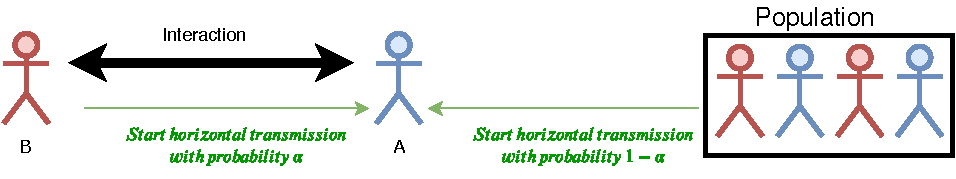
\includegraphics[scale=1]{figure.pdf}
  \caption{\textbf{Cultural horizontal transmission.} Transmission occurs between interaction partners with probability $\alpha$ (left) or between two random peers with probability $1-\alpha$.}
  \label{fig:horizontal}
\end{figure}

\section*{Results}

We start by inspecting specific cases, for which we can derive general results. 
Afterwards, we use numerical simulation to analyze more complex cases.

\paragraph*{Without oblique transmission, $v=1$.} 
With only vertical transmission eq.~\ref{eq:vertical_oblique_transmission} becomes
$\hat{p} =  \tilde{p}$,
and eq.~\ref{eq:nextgen_parents} for the change in frequency $p'$ of phenotype $A$ among parents can be written as

\begin{equation} 
\begin{split}\label{eq:nextgen_parents_vertical_only}
\bar{w} \tilde{p}' 
& = p^2 (1+b-c) (1 - (1-p) (1-\alpha) T_B) \\
& + p(1-p) (1-c) (p (1-\alpha) T_B + 1 - T_B) \\
& + p(1-p) (1+b) (p (1-\alpha) + \alpha) T_A \\
& + (1-p)^2 p (1-\alpha) T_A
\end{split}
\end{equation}

\textbf{Result 1.}
If 
\begin{equation}\label{result1}
c \cdot (1-T_B) < b \cdot  \alpha T_A  + (T_A - T_B) [1 + b (p(1-\alpha) - 1)]
\end{equation}
then $\tilde{p}' > \tilde{p}$, and the frequency of phenotype $A$ among parents increases. 

\textbf{Corollary 1.1: equal horizontal transmission.}
If $T=T_A=T_B$, then
\begin{equation}
\label{eq:equal_transmission}
\frac{1-T}{\alpha T} < \frac{b}{c},
\end{equation}
which can be seen as a cultural version of \emph{Hamilton's rule} (eq.~\ref{eq:hamilton_rule}).

%(yr: I stopped here)
	
\underline{Special case 2 - $\alpha =1$:} in this case, horizontal transmission can only occur as a result of interaction.
\\Eq. \eqref{result0} becomes:
\begin{equation} 
\begin{split} \label{result3}
c(1-T_B)  < & \, T_A -T_B +b(T_A-T_B)
\end{split}
\end{equation}
Therefore, cooperative behavior will take over the population when eq. \eqref{result3} is satisfied. 
This result is in accordance with the result presented by Lewin-Epstein at el. \cite{Ohad}. 
\\\underline{Special case 3 - $\alpha = 0$:} in this case horizontal transmission can not occur as a result of interaction.  
Then, eq. \eqref{result0} becomes:
\begin{equation} 
\begin{split} \label{result4}
0 < & \,  - bq(1-T_B)- bT_B-c(1-T_B)-T_B
\end {split}
\end{equation}
Which is always false because all of the elements are negative. Therefore, cooperation will eventually disappear from population.
\\Those are the results we have so far. However, there is a still work need to be done. \\
We will analyze the equilibrium points in this model. We know that $p=1$ is an equilibrium point because if the all individuals in the population are cooperators then in next generation all individual will be cooperator as well. Same for $p=0$. We will check if there are any more equilibrium points. For each equilibrium point we will determine whether it is stable equilibrium or not. 
\\So far, we assumed that $v=1$. We believe it will be interesting to test the effect of oblique transmission ($v\neq 1$) since oblique transmission is common in cultural evolution models. Therefore, we are planning to simulations to investigate the case when $v\neq 1$. 

\subsection*{Aim 2}
Prisoner's dilemma is widely studied and most of the models developed in order to learn about evolution of cooperation is using it as the model of interaction's result. However, often the reality is different. For example, interaction could be between than two individuals. 
In the first aim we hypothesize that non-vertical transmission can explain the evolution of cooperation in fully mixed population with prisoner's dilemma payoff. Here, we hypothesize that non-vertical transmission can also explain the evolution of cooperation in fully mixed population with other games. The second aim is to determine to what extent our hypothesize could explain the evolution of cooperation. We will develop and investigate a cultural evolution model like we did in the first aim but with different games. 
In the first scenario we can use n-player prisoner's dilemma a.k.a unscrupulous diner's dilemma or just diner's dilemma. The diner's dilemma is the main game we will investigate. In the diner's dilemma we assume that n players are eating in a restaurant. There are two dishes in the restaurant: dish1 with cost $c_1$ and benefit $b_1$ and dish2 with cost $c_2$ and benefit $b_2$. We also know that $b_2>c_2>b_1>c_1$. We presume that one would prefer to order the expensive meal given others will help defray the cost,
\begin{equation} 
\begin{split} \label{diner}
b_2-\frac{1}{n}c_2 >\, & b_1 - \frac{1}{n}c_1.
\end {split}
\end{equation}
Cooperative individual is an individual who choose to take the cheap dish. Choosing the cheap dish increases the fitness of the competitors. 
In the second scenario we can use public common goods as our game. Public common goods is a multiplayer game in which each player can secretly choose how much he want to contribute. The contributions from all players is collected and the sum is multiplied by a factor (greater or equal to one) and the result is the "public good". The public good is evenly divided among the players. A player will be considered as a cooperator if decide to contribute. 
In the third scenario, we want to use a general two player game. Prisoner dilemma is an example of a two player game with a payoff matrix shown in figure \ref{fig:payoff}. We will investigate the general case. The payoff matrix in the general case is shown in figure \ref{fig:generalPayoff}.
\begin{figure}[h!]
  \centering
  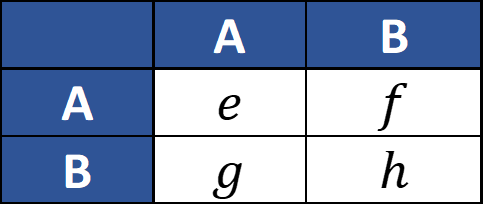
\includegraphics[scale=0.4]{generalpayoff.pdf}
  \caption{General Payoff Matrix}
  \label{fig:generalPayoff}
\end{figure}

\subsection*{Aim 3}
In the previous aims we focused in fully mixed populations. Many time in reality, the population is structured. When the population is spatially structured, individuals interact only with their neighbors, which are more likely to be related. Therefore, cooperators are more likely to interact with cooperators and vice versa. Here we hypothesize that non-vertical transmission can also explain the evolution of cooperation in spatially structured population. We will develop and investigate a cultural evolution model. 
we will analyse these models with simulations. 

\newpage
\section*{Conclusions}
We hypothesized that non-vertical transmission can explain the evolution of cooperation. We used a model with non-vertical transmissions and have found that if eq. \eqref{result} is satisfied cooperation will take over the population in fully mixed population with prisoner's dilemma payoff. In addition, we found that when horizontal transmission cannot occur after interaction ($\alpha = 0$) cooperation will always become extinct. 
Our results improve our understating of cultural evolution of cooperation. Our model shows that cooperation can evolve even in a fully mixed population, where the population is non-structured, there are no repeating interactions and nor individual recognition.

\bibliography{bib}


\newpage
\section*{Appendix A}
In the section, we start with eq. \eqref{modeleq} and we want to investigate when $p\leq p'$. We know that $0<p<1$ and $0<c<b$.

We start by multiple by $\overline{\omega}$ The result is shown in eq. \eqref{step1}.
\begin{equation} 
\begin{split} \label{step1}
p + p^2(b-c) < & \, \{ p^2(1+b-c)[1-(1-\alpha)T_Bq] + pq(1-c)[1-(1-\alpha)T_Bq-\alpha T_B)]\\
&+ pq(1+b)[\alpha T_A+(1-\alpha)T_Ap)] + q^2(1-\alpha)T_Ap\}
\end{split}
\end{equation}

Divining by p and substituting $p=1-q$ give us eq. \eqref{step2}
\begin{equation} 
\begin{split} \label{step2}
1 + (1-q)(b-c) < & \, \{ (1-q)(1+b-c)[1-(1-\alpha)T_Bq] + q(1-c)[1-(1-\alpha)T_Bq-\alpha T_B)]\\
&+ q(1+b)[\alpha T_A+(1-\alpha)T_A(1-q))] + q^2(1-\alpha)T_A\}
\end{split}
\end{equation}
Eq. \eqref{step2} becomes eq. \eqref{step3}.
%\begin{equation} 
%\begin{split} \label{step3}
%1 + b - c - q(b-c) < & \, \{ bq^2T_B-b\alpha q^2T_B - bq^2T_A + \alpha bq^2T_A - bq - qT_B - bqT_B + \alpha bqT_B +cqT_B + qT_A + bqT_B + b - c + 1 \}
%\end{split}
%\end{equation}
\begin{equation} 
\begin{split}\label{step3}
 -q(b-c) < & \,  bq^2T_B-b\alpha q^2T_B - bq^2T_A + \alpha bq^2T_A - bq - qT_B - bqT_B + \alpha bqT_B +cqT_B + qT_A + bqT_B 
\end{split}
\end{equation}

We can divide by q because we know that $0<q<1$ then,
\begin{equation} 
\begin{split} \label{step4}
 c(1-T_B) < & \,  bqT_B(1-\alpha) - bqT_A(1-\alpha) + (T_A-T_B) + b(T_A - T_B) + \alpha bT_B.
\end{split}
\end{equation}

In the special case when $T_A = T_B = T$ equation \eqref{step4} becomes
\begin{equation} 
\begin{split}\label{step5}
c(1-T) < & \, \alpha bT.
\end{split}
\end{equation}
Eq. \eqref{step5} can be rewritten as
\begin{equation} 
\begin{split}
 \frac{1-T}{\alpha T} < \frac{b}{c}.
\end{split}
\end{equation}


\end{document}
